\section{Experimental Setup}
To evaluate the effectiveness of our symmetry elimination technique we performed
a comparative analysis using A* on a number of benchmarks taken from
the freely available pathfinding library 
Hierarchical Open Graph (HOG)\footnote{\url{http://www.googlecode.com/p/hog2}}:
\begin{itemize}
\item{\textbf{Adaptive Depth} is a set of 12 maps of size 100$\times$100 in which approximately
$\frac{1}{3}$ of each map is divided into adjacent rectangular rooms of
varying size and the rest of the map is a large open area interspersed with 
large randomly placed obstacles.}
\item{\textbf{Baldur's Gate} is a set of 120 maps taken from BioWare's popular
roleplaying game \emph{Baldur's Gate II: Shadows of Amn}. 
Often appearing as a standard benchmark in the literature 
\cite{botea04,bjornsson05,bjornsson06,sturtevant05,harabor08} these maps range in 
size from 50$\times$50 to 320$\times$320 and have a distinctive 45-degree orientation.
Figure \ref{fig-bgmap} shows a typical example.}
\item{\textbf{Rooms} is a set of 300 maps of size 256$\times$256 which are divided into 32$\times$32
rectangular areas that are connected by randomly placed entrances.}
\end{itemize}

 \begin{figure}[t]
        \begin{center}
                        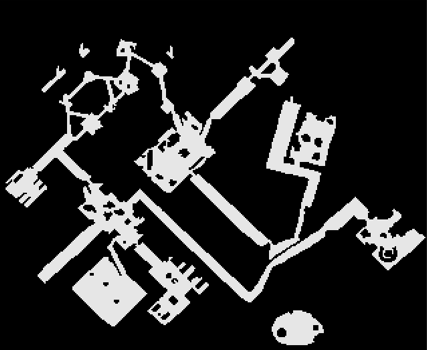
\includegraphics[width=0.6\columnwidth, trim = 10mm 10mm 10mm 0mm]{diagrams/bgmap.png}
        \end{center}
        \caption{A map from BioWare's \emph{Baldur's Gate II}}
        \label{fig-bgmap}
 \end{figure}
\par
For each map we removed all diagonal edges and randomly generated 100 valid problem instances. 
We then ran A* twice: once on the original maps and again on our modified maps making for
a total of 86400 (432$\times$100$\times$2) distinct experiments.
Our test machine had a 2.93GHz Intel Core 2 Duo processor, 4GB RAM and
ran OSX 10.6.2.
We use the A* implementation provided in HOG.
